\chapter{METODE PENENILITIAN}

\section{Garis Besar Penelitian}

\noindent Secara garis besar, penelitian ini akan melaksanakan pengembangan sistem monitoring mesin diesel berbasis \textit{IoT} yang akan diuji pada PT Bisma Jaya untuk meningkatkan efektivitas operasi dengan menekankan kecepatan minimum pada armada dan efisiensi biaya bahan bakar dengan memantau jumlah bahan bakar yang digunakan setiap harinya. Tampilan web akan dikembangkan menggunakan framework NextJS berbasis JavaScript dan sistem \textit{backend} menggunakan framework Django berbasis Python. Pengembangan sistem ini akan menggunakan metode Extreme Programming yang memiliki tahapan sebagai berikut: Exploration Phase, Planning Phase, Iteration to Release Phase, Productionizing Phase, Maintenance Phase, dan Death Phase. 

\section{Diagram Alir Penelitian}

\noindent Metodologi pelaksanaan penelitian ini dapat dimodelkan menggunakan diagram alir sebagai berikut.

\begin{figure}[!h]
    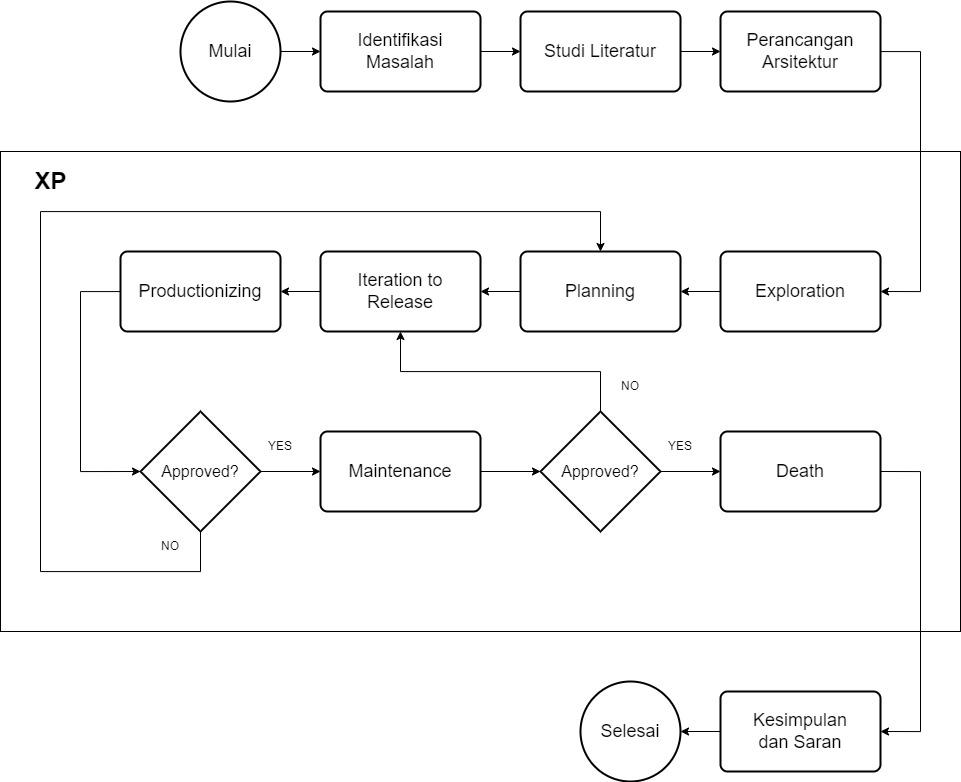
\includegraphics[width=1.1\linewidth, center]{images/metode/flowchart-penelitian.jpg}
    \caption{Diagram Alir Penelitian}
    \label{fig:flow-research}
\end{figure}


Pada Gambar 3.1 dapat dilihat bahwa penelitian ini diawali dengan melakukan identifikasi masalah dan studi literatur mengenai jurnal-jurnal dari penelitian relevan yang telah dilakukan sebelumnya. Kemudian, dilanjutkan dengan pengembangan sistem menggunakan metode \textit{Exteme Programming (XP)} yang terdiri dari Exploration Phase, Planning Phase, Iteration to Release Phase, Productionizing Phase, Maintenance Phase, dan Death Phase. Terakhir dilakukan pembuatan kesimpulan dan saran dari penelitian.

\section{Prosedur Penelitian}

\noindent Berikut penjelasan prosedur penelitian secara rinci berdasarkan tahapan-tahapan yang ditetapkan pada Gambar 3.1 sebagai pedoman penelitian ini.

\begin{enumerate}
    \item \textbf{Identifikasi Masalah}
    
    Penelitian ini dimulai dengan mengidentifikasi permasalahan yang ada di mitra. Ini dilakukan melalui dua cara, diskusi dengan seluruh \textit{stakeholder} yang terlibat dan observasi ke lapangan. Dari tahap ini akan dihasilkan rumusan masalah, tujuan, serta batasan-batasan penelitian.

    \item \textbf{Studi Literatur}
    
    Pada tahap ini dilakukan studi literatur dengan mengumpulkan berbagai referensi yang didapat dari jurnal, artikel ilmiah, dan sumber lainnya mengenai pengembangan sistem berbasis \textit{IoT}, teknologi-teknologi yang digunakan selama penelitian, dan perbandingan metodologi dalam pengembangan perangkat lunak.

    \item \textbf{Pengembangan Sistem}
    
    \begin{enumerate}[label*=\arabic*.]
        \item \textbf{Perancangan Arsitetur}
        \item \textbf{Extreme Programming}
        
        \begin{enumerate}[label*=\arabic*.]
            \item \textbf{\textit{Exploration Phase}}
            
            Kebutuhan yang dikumpulkan pada tahap identifikasi masalah kemudian dibuat dalam bentuk \textit{user story} untuk mendeskripsikan hasil yang diinginkan. Daftar \textit{user story} sementara dapat dilihat pada tabel berikut.

            \begin{longtable}[!h]
                {
                    p{0.15\textwidth}
                    p{0.15\textwidth}
                    p{0.35\textwidth}
                    p{0.35\textwidth}
                }
                    \toprule
                    \textit{Code} & 
                    \textit{Persona} & 
                    \textit{I want to} &
                    \textit{So that can} \\ [0.5ex] 
                    \midrule
                    
                    US-01 & 
                    \textit{User} & 
                    \textit{Login} & 
                    Mengakses sistem sesuai dengan username dan password 
                    \\  
                    
                    US-02 & 
                    \textit{User} & 
                    \textit{Logout} & 
                    Keluar dari sistem melalui tombol logout \\  
                    
                    US-03 & 
                    \textit{User} & 
                    Melihat data historis kecepatan mesin & 
                    Memastikan armada bergerak dengan kecepatan mesin yang sesuai
                    \\  
                    
                    US-04 & 
                    \textit{User} & 
                    Melihat data historis konsumsi bahan bakar &   
                    Melakukan kontrol bahan bakar
                    \\  
                    
                    US-05 & 
                    \textit{User} &     
                    Melihat data historis \textit{running hour} & 
                    Memastikan operasi berjalan dengan optimal
                    \\  
                    
                    US-06 & 
                    \textit{User} &         
                    Melihat data log kecepatan per menit &   
                    Melihat detail kecepatan pada waktu spesifik
                    \\  
                    
                    US-07 & 
                    \textit{User} &       
                    Mencetak laporan kecepatan mesin harian &     
                    Mendapatkan laporan harian kecepatan mesin dengan format PDF
                    \\  
                    
                    US-08 & 
                    \textit{User} &     
                    Mencetak laporan harian konsumsi bahan bakar & 
                    Mendapatkan laporan harian konsumsi bahan baar dengan format PDF 
                    \\  
                    
                    US-09 & 
                    \textit{User} &         
                    Mengunduh data log kecepatan mesin &     
                    Mendapatkan log kecepatan mesin dengan format CSV
                    \\ [1ex] 
                    \bottomrule
                \caption{User Story Sementara}
                \label{tab:user-story}
            \end{longtable}

            \item \textbf{\textit{Planning Phase}}
            
            User story yang dibuat pada tahap sebelumnya akan dikumpulkan dan disimpan berdasarkan prioritas di release plan. Tahap ini akan diulang kembali setelah melewati tahap testing sesuai dengan jumlah iterasi pengembangan.
            
            

            \item \textbf{\textit{Iteration to Release Phase}}
            
            Berdasarkan \textit{user story} yang dibuat di tahap sebelumnya, akan dilakukan perancangan \textit{user interface} sistem dan skema basis data dalam bentuk \textit{entity relationship diagram (ERD)} yang akan membantu dalam menggambarkan hubungan antar tabel. ERD sistem sementara dapat dilihat pada gambar berikut.

            \begin{figure}[!h]
                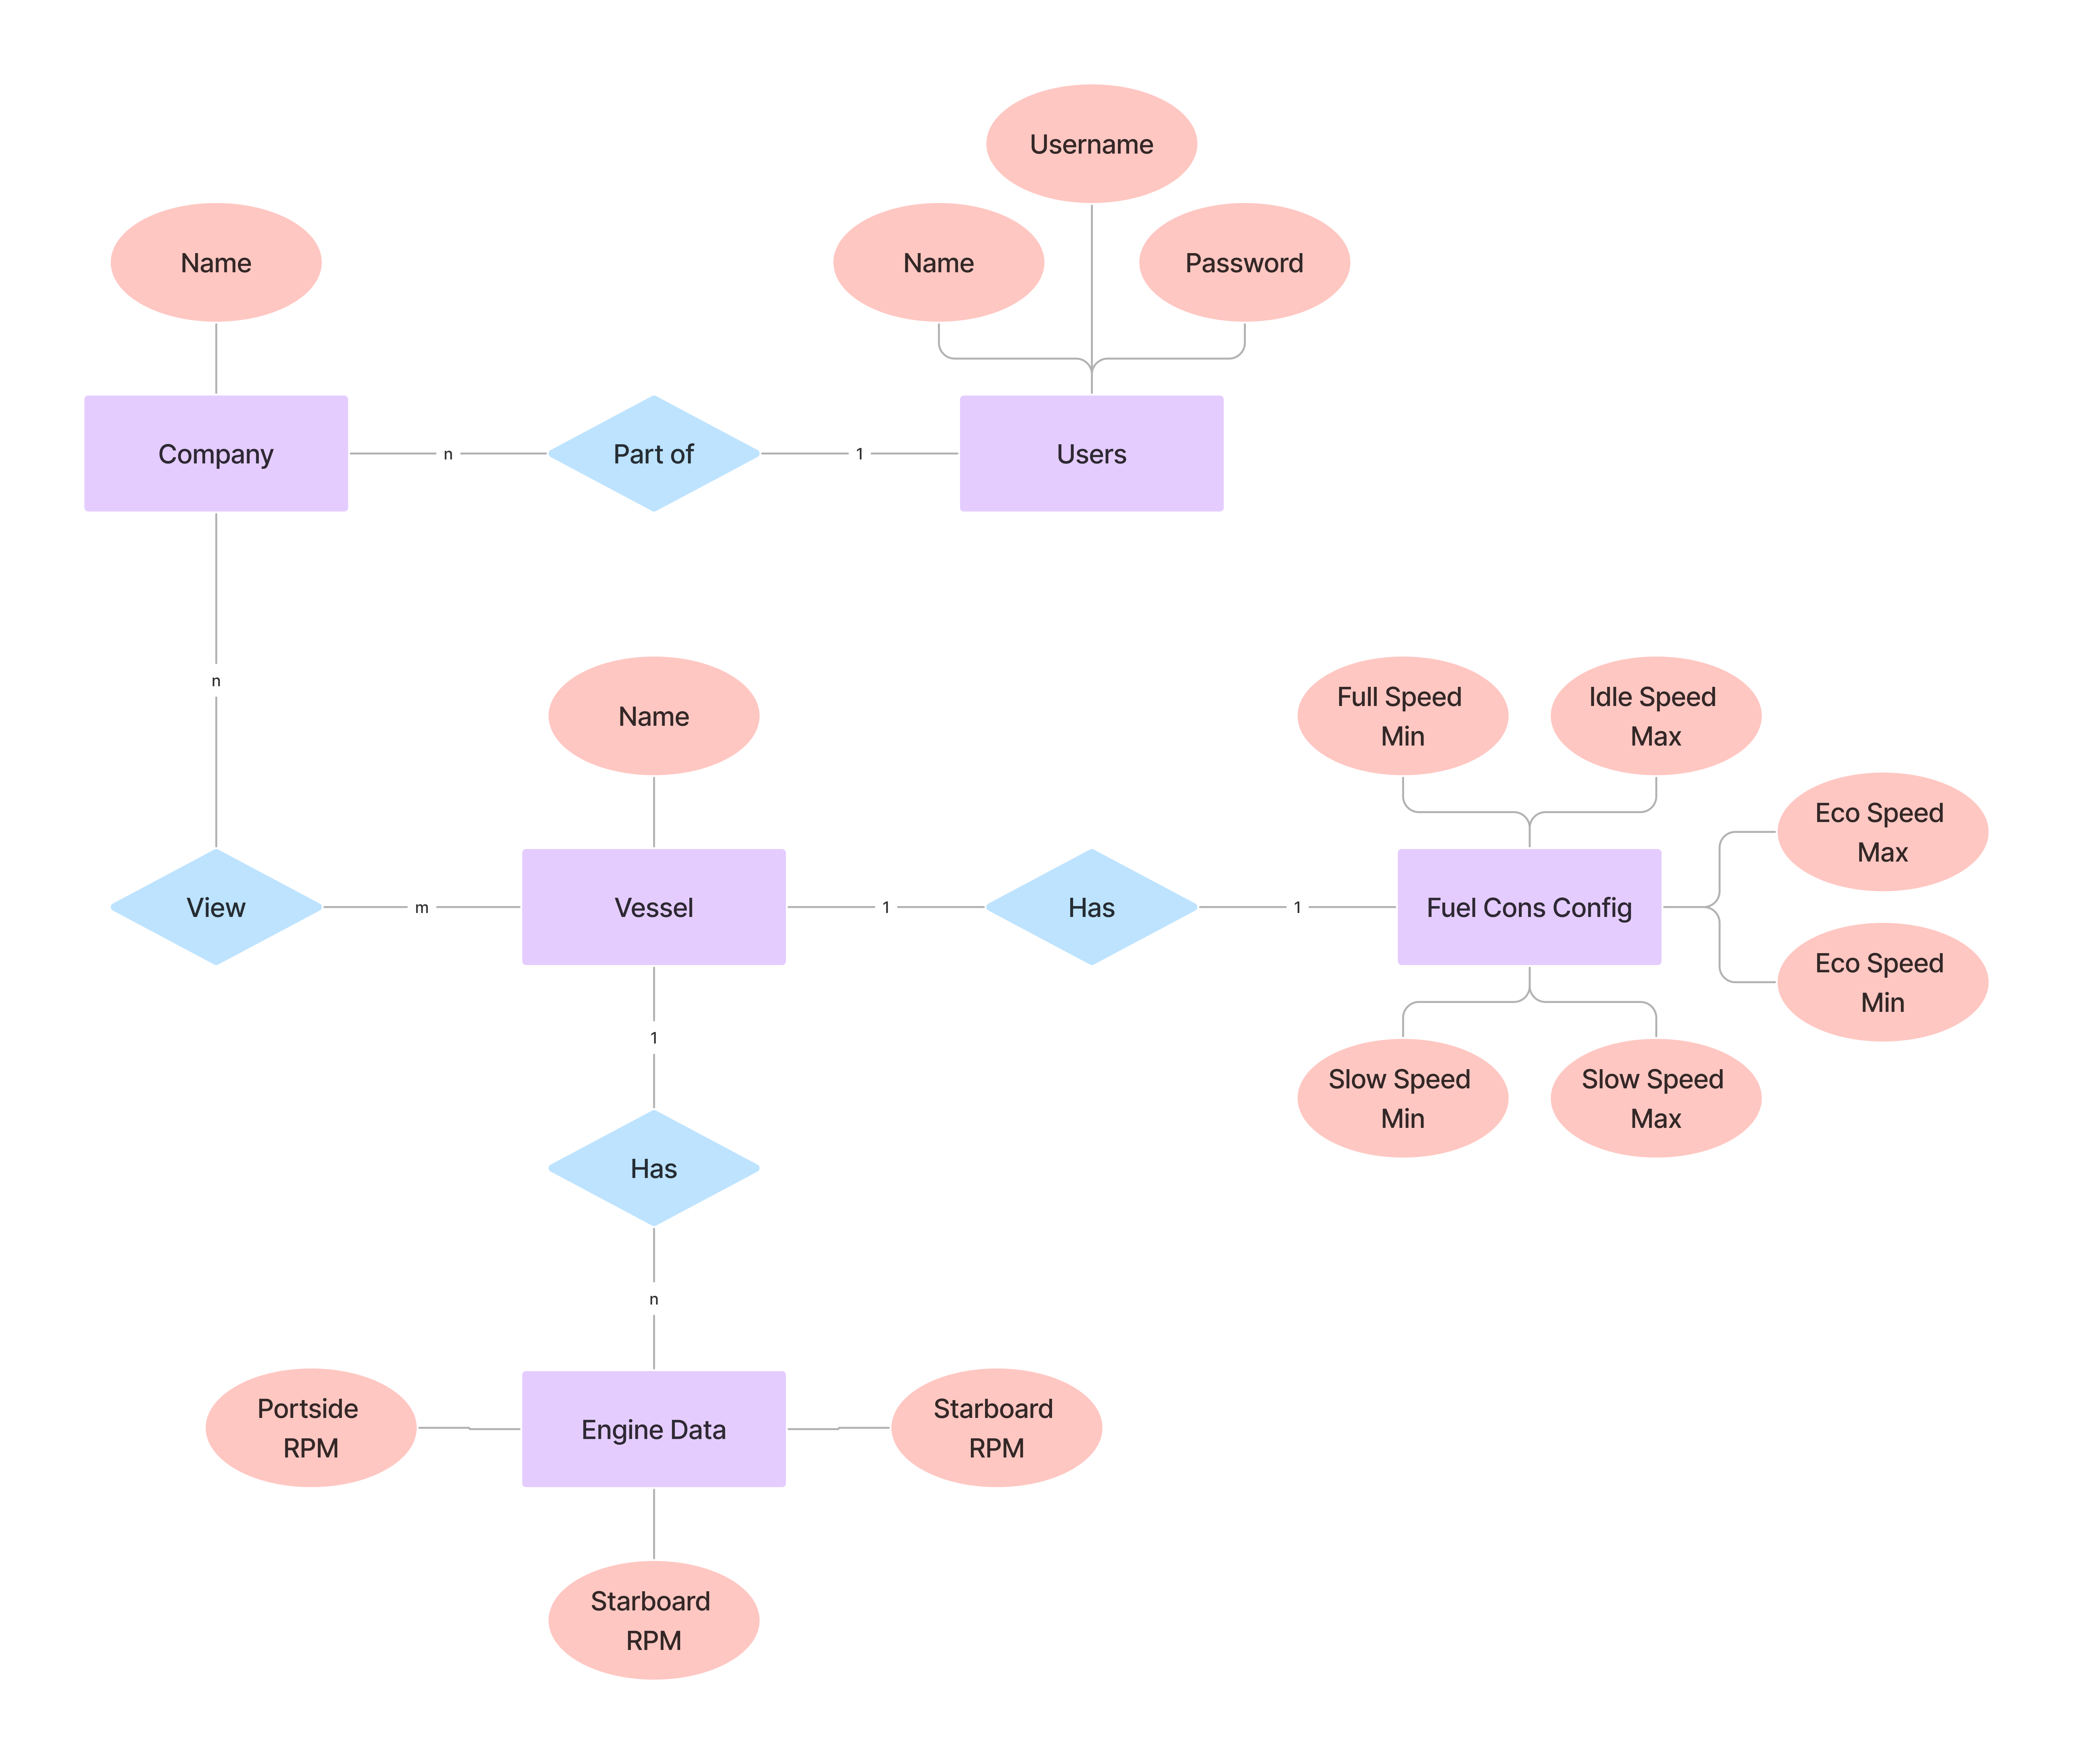
\includegraphics[width=1\linewidth, center]{images/metode/erd.png}
                \caption{Entity Relationship Diagram (ERD) Sementara}
                \label{fig:erd}
            \end{figure}

            Secara parallel, dilakukan tahap implementasi dari perancangan sistem. Dalam pengembangan dashboard digunakan framework NextJS untuk menghasilkan tampilan yang dinamis, kemudian digunakan framework Django yang berbasis bahasa Python untuk menghubungkan perangkat IoT dengan server. Setelah dilakukannya pengembangan pada satu iterasi, sistem akan diunggah ke repositori dan akan diuji setelahnya oleh mitra melalui metode black box testing. Jika terdapat umpan balik, maka tahapan akan diulang ke tahap desain untuk menyesuaikan permintaan mitra. Sebaliknya, jika mendapatkan persetujuan maka sistem akan masuk ke tahap berikutnya.

            \item \textbf{\textit{Productionizing Phase}}
            
            Setelah melewati pengujian dan mendapatan persetujuan mitra, sistem akan diluncurkan secara perlahan pada server dengan mode development. Fitur yang dirasa kurang lengkap atau ingin ditambahkan oleh mitra akan balik di tahap planning untuk dilakukan prioritas. Jika mendapatkan persetujuan, akan dilanjutkan ke tahap berikutnya.

            \item \textbf{\textit{Maintenance Phase}}
            
            Pada tahap ini, sistem sudah hampir matang dan menunggu persetujuan terakhir dari mitra. Jika ditemukan bug atau ketidak sesuaian pada sistem maka akan kembali ke tahap Iteration to Release.

            \item \textbf{\textit{Death Phase}}
            
            Ini merupakan tahap terakhir, apabila seluruh fitur pada sistem telah selesai dikembangkan dan sesuai dengan kebutuhan awal mitra maka dilakukan tahap peluncuran dimana akan digunakan VPS cloud hosting.
        
        \end{enumerate}
    \end{enumerate}
\end{enumerate}

\section{Rencana Jadwal Penelitian}

\noindent Berikut jadwal penelitian yang disusun berdasarkan metodologi yang telah dijelaskan.

\begin{figure}[!h]
    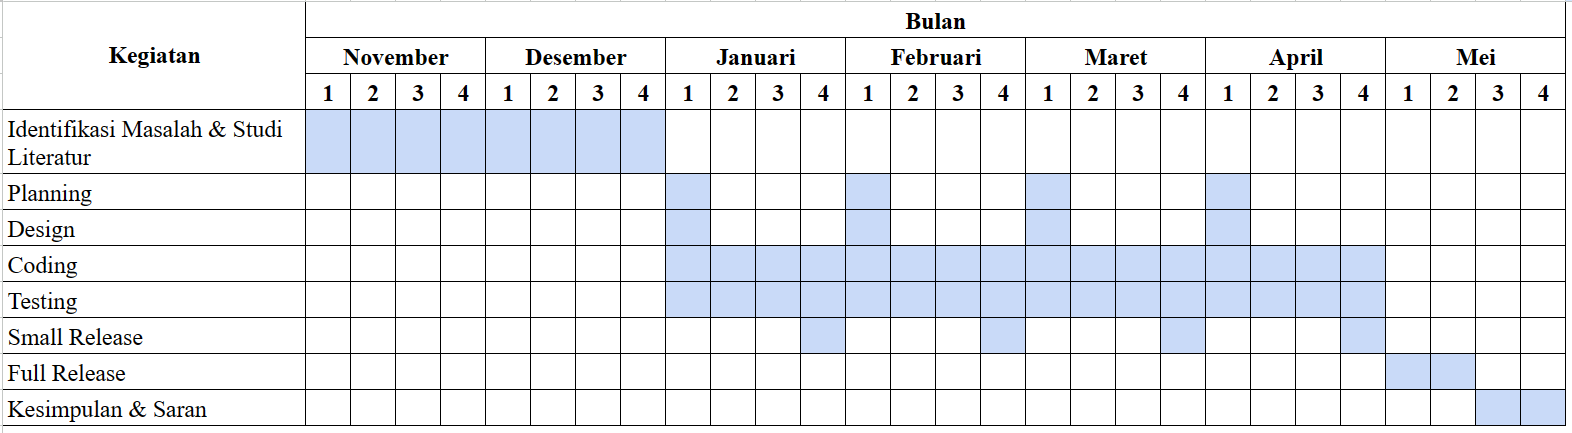
\includegraphics[width=1.2\linewidth, center]{images/metode/schedule.png}
    \caption{Rencana Jadwal Penelitian}
    \label{fig:flow-schedule}
\end{figure}